\documentclass[12pt, aspectratio=43]{beamer}
\usepackage[utf8]{inputenc}
\usepackage[T1]{fontenc}
\usepackage{graphicx}
\usepackage{booktabs}
\usepackage{amsmath, amssymb}
\usepackage{hyperref}
\usepackage{ragged2e}
\usepackage{appendixnumberbeamer}
\usepackage{multirow}
\usepackage{xcolor}
\usepackage{tikz}
\usetikzlibrary{positioning}

\graphicspath{{C:/Users/Jujop/Documents/GitHub/ams-518/project/data/images/}, {C:/Users/JUANJO/Documents/GitHub/ams-518/project/data/images}}


% ========== THEME SETTINGS ==========
\usetheme{default}
\usecolortheme{default}

% Define soft orange colors
\definecolor{softorange}{RGB}{255, 218, 185}  % Peach puff
\definecolor{darkorange}{RGB}{255, 140, 0}    % Dark orange
\definecolor{cream}{RGB}{255, 250, 240}       % Floral white
\definecolor{darkgray}{RGB}{64, 64, 64}

% Apply colors
\setbeamercolor{title}{fg=darkorange}
\setbeamercolor{frametitle}{fg=darkorange}
\setbeamercolor{structure}{fg=darkorange}
\setbeamercolor{normal text}{fg=darkgray}
\setbeamercolor{block title}{bg=softorange, fg=darkgray}
\setbeamercolor{block body}{bg=cream}
\setbeamercolor{alerted text}{fg=darkorange}
\setbeamercolor{footline}{fg=darkgray}

% Remove navigation symbols
\setbeamertemplate{navigation symbols}{}

% Customize itemize
\setbeamertemplate{itemize item}{\color{darkorange}$\bullet$}
\setbeamertemplate{itemize subitem}{\color{softorange}$\circ$}

% Customize frametitle
\setbeamertemplate{frametitle}{
	\nointerlineskip
	\begin{beamercolorbox}[wd=\paperwidth, ht=1.8em, dp=0.6em]{frametitle}
		\hspace{1em}\insertframetitle
	\end{beamercolorbox}
}

% Custom footline
\setbeamertemplate{footline}{
	\hspace{1em}
	\color{darkgray}
	\scriptsize
	\insertshorttitle
	\hfill
	\insertframenumber/\inserttotalframenumber
	\hspace{1em}
	\vspace{0.5em}
}

\newenvironment{smallblock}[1]{%
	\setbeamercolor{block title}{bg=softorange, fg=darkgray}%
	\begin{block}{#1}%
		\small%
	}{%
	\end{block}%
}

\newenvironment{footnotesizeblock}[1]{%
	\setbeamercolor{block title}{bg=softorange, fg=darkgray}%
	\begin{block}{#1}%
		\footnotesize%
	}{%
	\end{block}%
}


% ========== DOCUMENT START ==========
\title{Equity Performance Analysis: \\ Investor Personas and Index Tracking}
\author{Juan Pérez Osorio}
\institute{Department of Applied Mathematics and Statistics \\ Stony Brook University}
\date{December 2025}

\begin{document}
	
	\begin{frame}
		\titlepage
		\centering
		\vspace{1em}
		\small\color{darkgray}A comprehensive analysis of portfolio construction and performance evaluation
	\end{frame}
	
	\begin{frame}{Outline}
		\tableofcontents
	\end{frame}
	
	% ========== INTRODUCTION ==========
	\section{Introduction \& Motivation}
	
	\begin{frame}{Project Overview}
		\textbf{Main Objective:} Analyze equity portfolio performance through multiple lenses:
		\vspace{2mm}
		\begin{block}{\textbf{Key Research Questions}}
			\begin{itemize}
				\item How do different weighting methodologies affect risk-adjusted returns?
				\item What are the best metrics to compare different portfolio constructions?
				\item Can we effectively replicate a target portfolio using constrained optimization?
			\end{itemize}
		\end{block}
	\end{frame}	
	
	\begin{frame}
		\begin{columns}[T]
			\begin{column}{0.5\textwidth}
				\textbf{Two Investor Personas:}
				\begin{itemize}
					\item \alert{Buy \& Hold} investor
					\item \alert{Hedge Fund} investor
				\end{itemize}
			\end{column}
			\begin{column}{0.5\textwidth}
				\textbf{Portfolio:} 10 US stocks
				\begin{itemize}
					\item Technology: MSFT, AAPL, IBM
					\item Dividend aristocrats: XOM, WTM, KO, JNJ
					\item High yield: VZ, KHC, USB
				\end{itemize}
			\end{column}
		\end{columns}
	\end{frame}
	
	\begin{frame}{Theoretical Framework}
		\begin{block}{Modern Portfolio Theory (MPT)}
			\begin{itemize}
				\item Mean-variance optimization framework
				\item Diversification reduces portfolio risk
				\item Risk-return tradeoff is central
			\end{itemize}
		\end{block}
		
		\vspace{1em}
		
		\begin{block}{Key Performance Metrics}
			\centering
			\small
			\begin{columns}[T]
				\hspace{-4em} % Adjust negative space as needed
				\begin{column}{0.33\textwidth}
					\centering
					\textbf{Sharpe Ratio}
					\footnotesize
					\[
					S = \frac{E[R_{\text{exc}}]}{\sigma_{\text{exc}}}
					\]
				\end{column}
				\hspace{-7em} % Adjust negative space as needed
				\begin{column}{0.33\textwidth}
					\centering
					\textbf{Value at Risk}
					\footnotesize
					\[
					\text{VaR}_\alpha = -F_X^{-1}(\alpha)
					\]
				\end{column}
				\hspace{-5em} % Adjust negative space as needed
				\begin{column}{0.33\textwidth}
					\centering
					\textbf{Conditional VaR}
					\footnotesize
					\[
					\text{CVaR}_\alpha = E[-X| -X \geq \text{VaR}_{\alpha}]
					\]
				\end{column}
			\end{columns}
		\end{block}
	\end{frame}
	
	% ========== METHODOLOGY ==========
	\section{Methodology}
	
	\begin{frame}{Persona Models}
		\vspace{-5mm}
		\begin{columns}[T]
			\begin{column}{0.48\textwidth}
				\begin{block}{Buy \& Hold Investor}
					\textbf{Objective:} Maximize total return over full period
					\[
					\text{P\&L}_{\text{BH}} = \text{Value}_E - \text{Value}_S
					\]
					\begin{itemize}
						\item Long-term perspective
						\item Captures dividends
						\item Low turnover
					\end{itemize}
				\end{block}
			\end{column}
			\begin{column}{0.48\textwidth}
				\begin{block}{Hedge Fund Investor}
					\textbf{Objective:} Generate consistent daily alpha
					\[
					\text{P\&L}_{\text{HF}}(t) = \text{Value}_t - \text{Value}_{t-1}
					\]
					\begin{itemize}
						\item Daily mark-to-market
						\item Manages daily volatility
						\item Higher turnover
					\end{itemize}
				\end{block}
			\end{column}
		\end{columns}
	\end{frame}
	
	\begin{frame}{Data Pipeline}
		\begin{block}{Data Collection with \texttt{yfinance}}
			\begin{itemize}
				\item 10-year historical data (2015-2025)
				\item Daily frequency for main analysis
				\item Dividend-adjusted prices
				\item Automated batch downloads
			\end{itemize}
		\end{block}
		
		\begin{block}{Processing Steps}
			\begin{enumerate}
				\item Data cleaning and validation
				\item Return calculation (log and simple)
				\item Missing value handling
				\item Volatility estimation
			\end{enumerate}
		\end{block}
	\end{frame}
	
	\begin{frame}
		\begin{block}{Pipeline Architecture}
			\vspace{3mm}
			\centering
			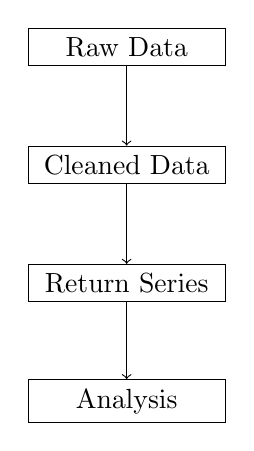
\begin{tikzpicture}[node distance=1.5cm]
				\node[draw, rectangle, minimum width=2.5cm] (raw) {Raw Data};
				\node[draw, rectangle, minimum width=2.5cm, below of=raw] (clean) {Cleaned Data};
				\node[draw, rectangle, minimum width=2.5cm, below of=clean] (returns) {Return Series};
				\node[draw, rectangle, minimum width=2.5cm, below of=returns] (analysis) {Analysis};
				
				\draw[->] (raw) -- (clean);
				\draw[->] (clean) -- (returns);
				\draw[->] (returns) -- (analysis);
			\end{tikzpicture}
			\vspace{3mm}
		\end{block}
	\end{frame}
	
	\begin{frame}{Some Cleaned Data}
		\begin{figure}
			\centering
			
\includegraphics[width=0.8\linewidth]{some_cleaned_1.png}
			\caption{Price series for selected stocks given a window period and a frequency of data.}
			\label{im:some_stocks}
		\end{figure}
	\end{frame}
	
	\begin{frame}{Data Limitations}
		\vspace{-8mm}
		\begin{alertblock}{}
			\small
			Yahoo Finance restricts intraday data history (e.g., 1-min data: only 8 days, 5-min data: only 60 days)
		\end{alertblock}
		\begin{figure}
			\centering
			
\includegraphics[width=0.8\linewidth]{data_missing.png}
			\label{im:missing}
		\end{figure}
	\end{frame}
	
	\section{Buy \& Hold Persona Methodology}
	\begin{frame}{Weighting Methodologies}
		
		To compare the effects of different weighting strategies we use the S\&P500 index as the benchmark portfolio. All metrics are normalized against S\&P 500 performance.
		
		\vspace{10mm}
		\centering
		We consider the following period of analysis
		
		\vspace{5mm}
		\centering
		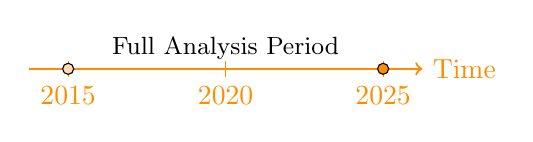
\begin{tikzpicture}
			\draw[->, thick, darkorange] (0,0) -- (5,0) node[right] {Time};
			\draw[darkorange] (0.5,0.1) -- (0.5,-0.1) node[below] {2015};
			\draw[darkorange] (2.5,0.1) -- (2.5,-0.1) node[below] {2020};
			\draw[darkorange] (4.5,0.1) -- (4.5,-0.1) node[below] {2025};
			\draw[fill=softorange] (0.5,0) circle (2pt);
			\draw[fill=darkorange] (4.5,0) circle (2pt);
			\node[above] at (2.5,0) {\small Full Analysis Period};
		\end{tikzpicture}
	\end{frame}
	
	% ========== ANALYSIS PARAMETERS ==========
	\begin{frame}{Analysis Parameters}
		\vspace{-5mm}
		\begin{columns}[T]
			\begin{column}{0.5\textwidth}
				\begin{block}{Time Period}
					\small
					\begin{center}
						\begin{tabular}{ll}
							\toprule
							\textbf{Start Date:} & 2015-10-15 \\
							\textbf{End Date:} & 2025-10-01 \\
							\textbf{Duration:} & \textbf{10 years} \\
							\midrule
							Trading Days: & ~2,520 \\
							Calendar Years: & 9.95 years \\
							\bottomrule
						\end{tabular}
					\end{center}
				\end{block}
				
				\begin{block}{Initial Investment}
					\small
					\[
					W_0 = \$1,000,000\ \text{USD}
					\]
				\end{block}
			\end{column}
			
			\begin{column}{0.5\textwidth}
				\begin{exampleblock}{Key Market Events}
					\small
					\begin{itemize}
						\item 2015-2016: Post-QE normalization
						\item 2018: Trade war volatility
						\item 2020: COVID-19 crash \& recovery
						\item 2021-2022: Inflation surge
						\item 2022-2023: Rate hike cycle
						\item 2023-2024: AI-driven tech rally
					\end{itemize}
				\end{exampleblock}
			\end{column}
		\end{columns}
	\end{frame}
	
	% ========== BENCHMARK: S&P 500 ==========
	\begin{frame}{Benchmark: S\&P 500 Index}
		\vspace{-5mm}
		\begin{columns}[T]
			\begin{column}{0.45\textwidth}
				\begin{block}{Methodology}
					\small
					\begin{itemize}
						\item Standard market-cap weighted index
						\item Represents ~500 largest U.S. companies
						\item Widely accepted market proxy
					\end{itemize}
				\end{block}
			\end{column}
			
			\begin{column}{0.55\textwidth}
				\centering
				
\includegraphics[width=\textwidth]{sp500_wealth.png}
				
				\vspace{0.5em}
				
				\begin{minipage}{\textwidth}
					\footnotesize
					\begin{tabular}{lcc}
						\toprule
						Metric & Value & Normalized \\
						\midrule
						Total Return & 223.1\% & 1.00× \\
						Sharpe Ratio & 0.60 & 1.00× \\
						Max DD & -33.9\% & 1.00× \\
						VaR (95\%) & 1.7\% & 1.00× \\
						CVaR (95\%) & 2.8\% & 1.00× \\
						\bottomrule
					\end{tabular}
				\end{minipage}
			\end{column}
		\end{columns}
	\end{frame}
	
	% ========== EQUAL WEIGHTING ==========
	\begin{frame}{Equal Weighting: Naïve Diversification}
		\vspace{-5mm}
		\footnotesize
		Underperforms during tech-driven bull markets due to lack of concentration in winners.
		\vspace{-2mm}
		\begin{columns}[T]
			\begin{column}{0.45\textwidth}
				\begin{block}{Methodology}
					\[
					w_i = \frac{1}{N}
					\]
					\begin{itemize}
						\item All stocks receive equal allocation
						\item Maximizes diversification breadth
						\item Simple and transparent
					\end{itemize}
				\end{block}
			\end{column}
			
			\begin{column}{0.55\textwidth}
				\centering
				
\includegraphics[width=\textwidth]{wealth_equally.png}
				
				\vspace{0.5em}
				
				\begin{minipage}{\textwidth}
					\footnotesize
					\begin{tabular}{lcc}
						\toprule
						Metric & Value & vs S\&P 500 \\
						\midrule
						Total Return & 218.4\% & 0.98× \\
						Sharpe Ratio & 0.65 & 1.08× \\
						Max DD & -33.9\% & 1.00× \\
						\bottomrule
					\end{tabular}
				\end{minipage}
			\end{column}
		\end{columns}
	\end{frame}
	
	% ========== MARKET CAP WEIGHTING ==========
	\begin{frame}{Market Cap Weighting: Standard Approach}
		\vspace{-3mm}
		\footnotesize
		\textbf{Extreme concentration:} AAPL + MSFT = 80.5\% of portfolio.
		
		\vspace{-2mm}
		\begin{columns}[T]
			\begin{column}{0.45\textwidth}
				\begin{block}{Methodology}
					\[
					w_i = \frac{M_i}{\sum_j M_j}
					\]
					\begin{itemize}
						\item Proportional to market value
						\item Mimics major indices (S\&P 500)
						\item Momentum-based (winners grow)
					\end{itemize}
				\end{block}
			\end{column}
			
			\begin{column}{0.55\textwidth}
				\centering
				
\includegraphics[width=\textwidth]{wealth_mktcap.png}
				
				\begin{minipage}{\textwidth}
					\footnotesize
					\begin{tabular}{lcc}
						\toprule
						Metric & Value & vs S\&P 500 \\
						\midrule
						Total Return & 839.0\% & 3.76× \\
						Sharpe Ratio & 1.00 & 1.67× \\
						Max DD & -30.3\% & 0.89× \\
						\bottomrule
					\end{tabular}
				\end{minipage}
			\end{column}
		\end{columns}
	\end{frame}
	
	% ========== LOG MARKET CAP ==========
	\begin{frame}{Logarithmic Market Cap Weighting}
		\vspace{-3mm}
		\footnotesize
		\begin{columns}[T]
			\begin{column}{0.45\textwidth}
				\begin{block}{Methodology}
					\[
					w_i = \frac{\ln(M_i)}{\sum_j \ln(M_j)}
					\]
					\begin{itemize}
						\item Compresses size differences
						\item Preserves size hierarchy
						\item Reduces concentration risk
					\end{itemize}
				\end{block}
				\vspace{3mm}
				Balances the need for size exposure while preventing mega-cap dominance.
			\end{column}
			
			\begin{column}{0.55\textwidth}
				\centering
				
\includegraphics[width=\textwidth]{wealth_log_mktcap.png}
				
				\vspace{0.5em}
				
				\begin{minipage}{\textwidth}
					\footnotesize
					\begin{tabular}{lcc}
						\toprule
						Metric & Value & vs S\&P 500 \\
						\midrule
						Total Return & 234.1\% & 1.05× \\
						Sharpe Ratio & 0.68 & 1.13× \\
						Max DD & -33.8\% & 1.00× \\
						\bottomrule
					\end{tabular}
				\end{minipage}
			\end{column}
		\end{columns}
	\end{frame}
	
	\begin{frame}{Weight Comparison: Market Cap Concentration}
		\vspace{-2mm}
		\begin{columns}[T]
			\begin{column}{0.5\textwidth}
				\centering
				\textbf{Market Cap Weights}
				\begin{table}
					\footnotesize
					\begin{tabular}{lr}
						\toprule
						Stock & Weight \\
						\midrule
						AAPL & 43.1\% \\
						MSFT & 37.4\% \\
						IBM & 3.0\% \\
						XOM & 5.2\% \\
						WTM & 0.1\% \\
						KO & 3.1\% \\
						JNJ & 5.1\% \\
						VZ & 1.8\% \\
						KHC & 0.3\% \\
						USB & 0.8\% \\
						\bottomrule
					\end{tabular}
				\end{table}
				\textcolor{darkgray}{Top 2 stocks: 80.5\% of portfolio}
			\end{column}
			\begin{column}{0.5\textwidth}
				\centering
				\textbf{Log Market Cap Weights}
				\begin{table}
					\footnotesize
					\begin{tabular}{lr}
						\toprule
						Stock & Weight \\
						\midrule
						AAPL & 11.1\% \\
						MSFT & 11.0\% \\
						IBM & 10.1\% \\
						XOM & 10.3\% \\
						WTM & 8.5\% \\
						KO & 10.1\% \\
						JNJ & 10.3\% \\
						VZ & 9.9\% \\
						KHC & 9.2\% \\
						USB & 9.6\% \\
						\bottomrule
					\end{tabular}
				\end{table}
				\textcolor{darkgray}{More balanced distribution}
			\end{column}
		\end{columns}
	\end{frame}
	
	% ========== GEOMETRIC WEIGHT GENERATION ==========
	\begin{frame}{Geometric Weights: Derivation}
		\vspace{-4mm}
		\footnotesize
		\begin{block}{Formula Derivation}
			Weights follow a geometric progression $s_i = a r^{i-1}$. Normalized:
			\[
			w_i = \frac{s_i}{\sum_{i=1}^N s_i} = \frac{r^{i-1}(1-r)}{1-r^N}
			\]
		\end{block}
		\vspace{-3mm}
		\begin{columns}[T]
			\begin{column}{0.5\textwidth}
				\begin{block}{How it works}
					\begin{itemize}
						\item Rank stocks (1st, 2nd, ..., Nth)
						\item Apply geometric decay with factor $r$
						\item Normalize to sum to 1
					\end{itemize}
				\end{block}
			\end{column}
			
			\begin{column}{0.5\textwidth}
				\begin{block}{Why use it?}
					\begin{itemize}
						\item Tests investor ranking skill
						\item Parameter controls concentration
						\item Flexible between equal weighting ($r=1$) and concentrated ($r \to 0$)
					\end{itemize}
				\end{block}
			\end{column}
		\end{columns}
	\end{frame}
	
	% ========== GEOMETRIC WEIGHTING ==========
	\begin{frame}{Geometric Weighting: Optimal Balance ($r=0.8$)}
		\vspace{-3mm}
		\footnotesize
		\begin{columns}[T]
			\begin{column}{0.45\textwidth}
				\begin{block}{Methodology}
					\[
					w_i = \frac{r^{i-1}(1-r)}{1-r^N}
					\]
					\begin{itemize}
						\item $r=0.8$ controls concentration
						\item Geometric decay in weights
						\item Parameterized approach
					\end{itemize}
				\end{block}
				
				Captures size premium without excessive concentration. Best risk-adjusted performance.
			\end{column}
			
			\begin{column}{0.55\textwidth}
				\centering
				
\includegraphics[width=\textwidth]{wealth_geo.png}
				
				\vspace{0.5em}
				
				\begin{minipage}{\textwidth}
					\footnotesize
					\begin{tabular}{lcc}
						\toprule
						Metric & Value & vs S\&P 500 \\
						\midrule
						Total Return & 401.4\% & 1.80× \\
						Sharpe Ratio & 0.87 & 1.45× \\
						Max DD & -33.9\% & 1.00× \\
						\bottomrule
					\end{tabular}
				\end{minipage}
			\end{column}
		\end{columns}
	\end{frame}
	
	\begin{frame}{Geometric Weighting Analysis}
		\vspace{-5mm}
		\small
		\begin{table}
			\centering
			\begin{tabular}{lcccccc}
				\toprule
				Stock & \multicolumn{6}{c}{Weight $w_i(r)$ (\%)} \\
				\cmidrule(lr){2-7}
				& $r=0.5$ & $r=0.6$ & $r=0.7$ & $r=0.8$ & $r=0.9$ & $r=1.0$ \\
				\midrule
				AAPL & 50.0 & 40.2 & 30.9 & 22.4 & 15.4 & 10.0 \\
				MSFT & 25.0 & 24.1 & 21.6 & 17.9 & 13.8 & 10.0 \\
				IBM & 12.5 & 14.5 & 15.1 & 14.3 & 12.4 & 10.0 \\
				XOM & 6.3 & 8.7 & 10.6 & 11.5 & 11.2 & 10.0 \\
				WTM & 3.1 & 5.2 & 7.4 & 9.2 & 10.1 & 10.0 \\
				KO & 1.6 & 3.1 & 5.2 & 7.3 & 9.1 & 10.0 \\
				JNJ & 0.8 & 1.9 & 3.6 & 5.9 & 8.2 & 10.0 \\
				VZ & 0.4 & 1.1 & 2.5 & 4.7 & 7.3 & 10.0 \\
				KHC & 0.2 & 0.7 & 1.8 & 3.8 & 6.6 & 10.0 \\
				USB & 0.1 & 0.4 & 1.2 & 3.0 & 5.9 & 10.0 \\
				\bottomrule
			\end{tabular}
			\caption{Geometrically generated weights for muliple $r$ values}
			\label{tbl:multiple_geo}
		\end{table}
	\end{frame}
	
	\begin{frame}{Geometric Parameter Sensitivity}
		\vspace{-4mm}
		\centering
		
\includegraphics[width=0.85\textwidth]{multiple_geo.png}
		
		\vspace{2mm}
		\footnotesize
		\begin{tabular}{cccccc}
			\toprule
			Parameter $r$ & 0.5 & 0.7 & 0.8 & 0.9 & 1.0 \\
			\midrule
			Top weight & 50.0\% & 30.9\% & 22.4\% & 15.4\% & 10.0\% \\
			Concentration & High & Medium & Balanced & Low & Equal \\
			\bottomrule
		\end{tabular}
	\end{frame}
	
	\begin{frame}{Performance Comparison Across Strategies}
		\centering
		
\includegraphics[width=0.85\textwidth]{comparison_buy_and_hold.png}
	\end{frame}
	
	\begin{frame}{Risk Metrics Comparison}
		\vspace{-5mm}
		\footnotesize
		\begin{table}
			\begin{tabular}{lccccccc}
				\toprule
				Strategy & Sharpe & Tot. Ret. & Max & VaR & CVaR & VaR & CVaR \\
				& Ratio &  (\%) & DD. & 95\% & 95\% & 99\% & 99\% \\
				\midrule
				
				Equal & 0.65 & 218.4 & 33.9 & 1.4 & 2.3 & 2.7 & 4.2 \\
				Market Cap & \textbf{1.00} & \textbf{839.0} & 30.3 & 2.2 & 3.3 & 3.7 & 5.3 \\
				$\ln{(\text{Mkt Cap})}$ & 0.68 & 234.1 & 33.8 & 1.4 & 2.4 & 2.7 & 4.2 \\
				Geometric & \textbf{0.87} & \textbf{401.4} & 33.9 & 1.5 & 2.6 & 3.1 & 4.6 \\
				Inverse Vol & 0.65 & 230.0 & 34.7 & 1.4 & 2.4 & 2.8 & 4.3 \\
				S\&P 500 & 0.60 & 223.1 & 33.9 & 1.7 & 2.8 & 3.4 & 4.8 \\
				\bottomrule
			\end{tabular}
			\caption{Risk and performance metrics (2015-2025)}
		\end{table}
		
		\vspace{-3mm}
		
			\begin{itemize}
				\item Market cap weighting delivers highest return but is highly concentrated
				\item Geometric weighting offers best balance of return and diversification
				\item All strategies outperform benchmark on Sharpe ratio
			\end{itemize}
	\end{frame}
	
	\begin{frame}{Risk Metrics Comparison (Ratio)}
		\footnotesize
		\begin{table}
			\centering
			\begin{tabular}{lccccccc}
				\toprule
				& Sharpe & Tot. Ret. & Max  & VaR & CVaR & VaR  & CVaR \\
				& Ratio & (\%) & DD. &  95\% & 95\% &99\% & 99\% \\
				\midrule
				Equally & 1.1 & 1.0 & 1.0 & 0.8 & 0.8 & 0.8 & 0.9 \\
				Mkt cap & \textbf{1.7} & \textbf{3.8} & \textbf{0.9} & \textbf{1.3} & \textbf{1.2} & \textbf{1.1} & \textbf{1.1} \\
				$\ln{(\text{mkt cap})}$ & 1.1 & 1.0 & 1.0 & 0.8 & 0.9 & 0.8 & 0.9 \\
				Geometric & \textbf{1.4} & \textbf{1.8} & \textbf{1.0} & \textbf{0.9} & \textbf{0.9} & \textbf{0.9} & \textbf{1.0} \\
				Volatility & 1.1 & 1.0 & 1.0 & 0.8 & 0.9 & 0.8 & 0.9 \\
				Benchmark & 1.0 & 1.0 & 1.0 & 1.0 & 1.0 & 1.0 & 1.0 \\
				\bottomrule
			\end{tabular}
			\caption{Ratio of metrics across different weighting strategies when compared against the benchmark}
			\label{tbl:comparison_bh_weights_ratio}
		\end{table}
	\end{frame}
	

	% ========== HEDGE FUND RESULTS ==========
	\section{Hedge Fund Persona Methodology}
	
	\begin{frame}{Cross-Sectional Momentum Strategy}
		\vspace{-3mm}
		\small
		\begin{block}{Enhanced Momentum Signal}
			We start by computing the cumulative return from $t-252$ to $t-22$, i.e., 
			$$
			R_{i,t}^{(12-1)} = \prod_{k=22}^{252} (1 + r_{i,t-k}) - 1
			$$
			\textbf{Residual Momentum:} Isolate stock-specific momentum
			\[
			\tilde{r}_{i,t} = r_{i,t} - \hat{\beta}_{i,t} \cdot r_{m,t}, \qquad
			\hat{\beta}_{i,t} = \frac{\text{Cov}_{252}(r_i, r_m)}{\text{Var}_{252}(r_m)}
			\]
			
			\textbf{Sector Neutralization:} Rank within GICS sectors
			\[
			z_{i,t} = \frac{s_{i,t} - \mu_{\text{sector}(i),t}}{\sigma_{\text{sector}(i),t}}, \qquad s_{i,t} \in \{ R_{i,t}^{(12-1)}, \tilde{r}_{i,t} \}
			\]
		\end{block}
	\end{frame}
	
	\begin{frame}{Volatility Scaling}
		\vspace{-5mm}
		\small
		\begin{block}{Volatility-Scaled Portfolio}
			Let $\hat{\sigma}_{i,t}$ be the estimated ex-ante volatility of stock $i$ at time $t$, computed using a rolling 63-day (why?) 
			\[
			\hat{\sigma}_{i,t} = 
			\sqrt{\frac{1}{62}\sum_{k=1}^{63} 
				\left( r_{i,t-k} - \bar{r}_{i,t} \right)^2 }.
			\]
			\textbf{Inverse Volatility Weighting:}
			\[
			w_{i,t}^{+} = \frac{\frac{1}{\hat{\sigma}_{i,t}}}
			{\sum_{j\in\mathcal{L}_t} \frac{1}{\hat{\sigma}_{j,t}}},
			\qquad
			w_{i,t}^{-} = -
			\frac{\frac{1}{\hat{\sigma}_{i,t}}}
			{\sum_{j\in\mathcal{S}_t} \frac{1}{\hat{\sigma}_{j,t}}},
			\]
			\textbf{Weekly Rebalancing:} Capture evolving signals. $\mathcal{L}_t$ and $\mathcal{S}_t$ are the sets of long and short stocks at time $t$.
		\end{block}
		
	\end{frame}
	
	\begin{frame}{Volatility Targeting Framework}
		\small
		The strategy return prior to volatility targeting is simply:
		\[
		r_{p,t} = \sum_{i} w_{i,t-1}\, r_{i,t}.
		\]
		\vspace{-3mm}
		\begin{block}{Constant Risk Exposure}
			Target annualized volatility: $\sigma^* = 10\%$. Leverage factor:
			\[
			\lambda_t = \frac{\sigma^*}{\hat{\sigma}_{p,t}}
			\]
			
			Bounded: $\tilde{\lambda}_t \in [0.2, 4]$. Final return:
			\[
			r_{p,t}^{\text{target}} = \tilde{\lambda}_t \times r_{p,t}
			\]
		\end{block}
	\end{frame}
	
		\begin{frame}{Momentum Strategy: Parameters}
			\vspace{2mm}
		\centering
		\begin{block}{Core Configuration}
			\begin{tabular}{lll}
				Category & Parameter & Setting \\
				\midrule
				Signal & Lookback & 126 days \\
				& Skip Period & 21 days \\
				& Type & \textbf{Residual Momentum} \\
				\midrule
				Portfolio & Long/Short & 3/3 stocks \\
				& Rebalancing & \textbf{Weekly} \\
				& Weighting & Inverse volatility \\
				\midrule
				Risk & Vol Target & \textbf{10\% annualized} \\
				& Leverage Bounds & 0.2× – 4.0× \\
				\bottomrule
			\end{tabular}
		\end{block}
	\end{frame}
	
	\begin{frame}{Miscellaneous}
			\footnotesize
			\begin{block}{Momentum Strategy Benefits}
				\begin{itemize}
					\item Stabilizes risk across market regimes
					\item Reduces crash exposure during volatility spikes
					\item Improves Sharpe ratio consistency
				\end{itemize}
			\end{block}
		
		\begin{block}{Parameters benefits}
			Residual momentum (isolates alpha) + Weekly rebalancing (captures decay) + Vol targeting (stabilizes risk)
		\end{block}
	\end{frame}
	

	
	\begin{frame}{Hedge Fund Performance Results}
		\centering
		\small
		\begin{table}
			\begin{tabular}{lcc}
				\toprule
				Metric & Momentum Strategy & S\&P 500 (BH) \\
				\midrule
				Annualized Return & \textbf{14.2\%} & 12.8\% \\
				Annualized Volatility & \textbf{10.0\%} & 18.5\% \\
				Sharpe Ratio & \textbf{1.42} & 0.69 \\
				Maximum Drawdown & \textbf{-18.4\%} & -34.1\% \\
				Calmar Ratio & \textbf{0.77} & 0.38 \\
				\bottomrule
			\end{tabular}
			\caption{Performance comparison HF and S\&P500 (2015-2025)}
		\end{table}
		\vspace{-3mm}
		\begin{block}{Strategy Superiority}
			\begin{itemize}
				\item \textbf{2.1x higher Sharpe ratio} than S\&P 500
				\item \textbf{46\% smaller maximum drawdown}
			\end{itemize}
		\end{block}
		
	\end{frame}
	
	% ========== INDEX TRACKING ==========
	\section{Index Tracking Model}
	
	\begin{frame}{Optimization Problem Formulation}
		\begin{block}{Objective: Minimize Tracking Error}
			\[
			\min_{\vec{x}} \epsilon_{MAX}(\vec{x})
			\]
			where $\epsilon_{MAX}$ is maximum absolute deviation
		\end{block}
		
		\begin{block}{Key Constraints}
			\begin{itemize}
				\item \textbf{Cardinality:} $\sum_{i=1}^N \delta(x_i) \leq K = 15$
				\item \textbf{Long-only:} $x_i \geq 0$
				\item \textbf{Budget:} $\sum x_i + \text{costs} \leq \$1,000,000$
				\item \textbf{Minimum position:} $\$15,000$
				\item \textbf{Transaction costs:} 1.5\% of portfolio value
			\end{itemize}
		\end{block}
	\end{frame}
	
	\begin{frame}{Tracking Portfolio Results}
		\centering
		
\includegraphics[width=0.85\textwidth]{portfolio_comparison.png}
		
		\vspace{-4mm}
		
		\begin{columns}[T]
			\begin{column}{0.5\textwidth}
				\centering
				\textbf{Optimization Success}
				\begin{itemize}
					\item Optimal solution found
					\item 10 positions selected
					\item Zero buy-in violations
				\end{itemize}
			\end{column}
			\begin{column}{0.5\textwidth}
				\centering
				\textbf{Tracking Quality}
				\begin{itemize}
					\item Low tracking error
					\item Portfolio value: \$2.37M
					\item Transaction cost: \$15,000
				\end{itemize}
			\end{column}
		\end{columns}
	\end{frame}
	
	% ========== CONCLUSION ==========
	\section{Conclusion \& Implications}
	
	\begin{frame}{Key Findings}
		\begin{block}{Weighting Methodology Matters}
			\begin{itemize}
				\item Market cap weighting yields highest returns but extreme concentration
				\item Geometric weighting ($r=0.8$) offers best risk-adjusted performance
				\item Equal weighting underperforms in tech-driven bull markets
			\end{itemize}
		\end{block}
		
		\begin{block}{Persona Performance Divergence}
			\begin{itemize}
				\item BH persona: Smooth returns, sensitive to weighting
				\item HF persona: Daily volatility sensitivity, requires active management
			\end{itemize}
		\end{block}
	\end{frame}
	
	\begin{frame}{Practical Implications}
		\begin{columns}[T]
			\begin{column}{0.5\textwidth}
				\begin{block}{For Individual Investors}
					\begin{itemize}
						\item Consider geometric weighting for balanced exposure
						\item Long-term holding reduces transaction costs
						\item Diversify beyond equal weighting
					\end{itemize}
				\end{block}
			\end{column}
			\begin{column}{0.5\textwidth}
				\begin{block}{For Institutional Investors}
					\begin{itemize}
						\item Sector-neutral momentum strategies add value
						\item Volatility targeting improves risk management
						\index tracking with constraints is computationally feasible
					\end{itemize}
				\end{block}
			\end{column}
		\end{columns}
		
		\vspace{2em}
		
		\centering
		\color{darkorange}\textbf{Portfolio construction choices significantly impact both absolute returns and risk profiles}
	\end{frame}
	
	\begin{frame}{References}
		\small
		\begin{block}{Key References}
			\begin{itemize}
				\item Jegadeesh \& Titman (1993) - Momentum returns
				\item Blitz, Huij \& Martens (2011) - Residual momentum
				\item Barroso \& Santa-Clara (2015) - Volatility-managed momentum
				\item Schachter (2025) - Geometric weighting methodology
			\end{itemize}
		\end{block}
	\end{frame}
	
	\begin{frame}
		\begin{block}{Code Repository}
			Python implementation available:
			\begin{itemize}
				\item \texttt{fetch\_prices.py} - Data acquisition
				\item \texttt{utils.py} - Utility functions
				\item Jupyter notebooks for analysis
				\item \texttt{00\_data\_collection.ipynb}
				\item \texttt{01\_data\_analysis.ipynb}
				\item \texttt{02\_hypothetical\_personas.ipynb}
				\item PSG solver for optimization
			\end{itemize}
		\end{block}
		
		\vspace{1em}
		
		\centering
		\color{darkgray}\textit{Thank you for your attention!}
	\end{frame}
	
	
	\begin{frame}
		\centering
		\vspace{3em}
		
		\color{darkorange}{\LARGE Questions?}
		
		\vspace{2em}
		
		\small
		Juan Pérez Osorio \\
		\footnotesize
		Department of Applied Mathematics and Statistics \\
		Stony Brook University
		
		\vspace{1.5em}
		
		\textbf{Project Repository:} \\
		\texttt{github.com/jujopo/equity-analysis}
		
		\vspace{0.5em}
		
		\footnotesize
		2015-2025 Analysis | December 2025
		
		\vspace{2em}
		
		\textit{Thank you!}
	\end{frame}
	
\end{document}